\chapter{Systém PerfEval}

\section{Popis systému}

S rozborem problematiky ve druhé kapitole je možné začít řešit programátorův
problém s vyhodnocováním výkonu popsaný ve scénáři z první kapitoly.
V důsledku toho je cílem vytvořit systém, který umožní porovnávat výsledky
měření výkonu, a který bude možné používat v rámci průběžné integrace.

Když už jsou známy požadavky na aplikaci, tak je možné ji začít navrhovat.
V této kapitole jsou popsané úvahy a rozhodnuté, které byly v průběhu vývoje
provedeny. Tyto úvahy a rozhodnutí vedly k tomu, že vyvinutý systém PerfEval je konzolová aplikace,
jejíž činnost je ovládaná příkazy a~parametry na~příkazové řádce.
Příkazy umožňují inicializovat systém, přidávat nové výsledky měření a~vyhodnocovat mezi sebou výsledky
měření dvou verzí.

\section{Rozbor alternativ v řešení}
Při~vývoji systému PerfEval došlo k~několika rozhodnutím, které výrazně ovlivnily jeho fungování a~architekturu.
Nejdůležitější rozhodnutí, která byla v~průběhu vývoje provedena, jsou v~následujících částech podrobně vysvětlena.

\subsection{Spouštění testů systémem PerfEval}
V~počátku vývoje bylo nutné se~rozhodnout, jakým způsobem bude systém přijímat a~zpracovávat výsledky testů.
V~úvahu přicházela varianta, že~uživatel provede měření výkonu sám, a~druhá varianta, že~uživatel systému
vysvětlí, jakým způsobem se~testování výkonu spouští. Pokud by byla zvolena varianta, kdy PerfEval spouští testy
sám, tak by bylo nutné nalézt dostatečně univerzální způsob spouštění testů.

Aplikace a~benchmarky pro měření výkonu mohou být jak konzolové, tak grafické aplikace. Pokud by PerfEval měl
měření provádět sám, tak by téměř určitě nebyl schopen pracovat s~grafickými aplikacemi, ale byl by schopen
spouštět programy s~parametry na~příkazové řádce.

Dále by bylo nutné vysvětlit, jak vypadá výstup spouštěných testů. Když pomineme formát, tak je nutné zjistit,
kam program, který provádí měření výsledky ukládá. Benchmarkovací systém BenchmarkDotNet například vypisuje
výsledky měření v podobě tabulky na standardní výstup a~zároveň ukládá strojově čitelné výsledky do~speciálního
k~tomu určeného adresáře.

Nakonec by to vypadalo tak, že při inicializaci systému uživatel zadá, jak spustit test výkonu a~kam se uloží výsledek.
Tímto způsobem by došlo k~tomu, že~PerfEval by začal určovat, jak mají vypadat programy, jejichž výstupy přijímá.
Na druhou stranu použití stávajícího řešení tyto nevýhody nemá. Jediné, co~musí uživatel zajistit, je, že~jeho
způsob měření zvládne uložit výsledek do~souboru, který PerfEval umí zpracovat.

Stávající řešení je tedy složitější v tom, že~uživatel musí testování výkonu spouštět sám. Poté, co~spustí testování
výkonu a~dostane soubor s~výsledky, jej přidá do databáze výsledků systému PerfEval a~poté spustí PerfEval s~příkazem evaluate
pro porovnání výsledků testování výkonu. Kdyby se použila varianta s~tím, že si PerfEval spouští testy sám, tak
by uživatel testování a~porovnání výkonu zvládl jedním spuštěním aplikace.

\subsection{Použité statistické metody}
Pro porovnání dvou výsledků měření se používají statistické metody. Statistické metody se používají ke zjištění,
jestli výsledky měření považované za~náhodné veličiny mají stejné rozdělení, popřípadě jestli je vzorků dostatečné množství.
V~systému PerfEval jsou implementovány statistické metody bootstrap a~t-test.

Pomocí bootstrapu dochází k~iluzi, že vzorků je mnohem více, než je jich ve skutečnosti změřeno. Protože měření vzorků
je samo o~sobě dlouhotrvající proces, tak se použití této statistické metody vyplatí. Bootstrap má ale tu nevýhodu, že jeho výpočet
může oproti prostému zkoumání vzorků trvat delší dobu.

t-test je tedy možné zvolit namísto bootstrapu kvůli tomu, že je rychlejší. Oproti náhodnému vybírání vzorků z~dvoudimenzionální sady
dat, kterým vzorky odpovídají, dochází k~pouhému dosazení hodnot do vzorce.

Uživatel by se tedy při volbě testu měl rozhodovat na základě toho kolik má změřených vzorků a~kolik má času na porovnání
výsledků měření. Pokud má uživatel naměřených vzorků málo a větší množství času k vyhodnocení doporučuje se použít bootstrap.
Pokud má uživatel větší množství vzorků a~málo času je pro něho lepší použít t-test.

\subsection{Rozpoznání formátu výsledků měření}

Systém, který porovnává výsledky měření výkonu, by měl mít informace o~tom v~jakém formátu jsou data uložena
a~který benchmarkovací framework je vytvořil. Podle použitého frameworku a~formátu je totiž možné výsledky
měření zpracovat pomocí programu a~transformovat data o~měření tak, aby jim systém rozuměl.
Problém je tedy jak se systém dozví o~tomto formátu a~o~použitém frameworku.

Nejpříjemnější řešení pro uživatele by bylo, že by systém sám přišel na to, který framework a~formát je použitý.
Uživatel by totiž nemusel vědět pomocí jakého frameworku a~v~jakém formátu data ukládá. Pro systém by však mohl
být problém různé frameworky rozlišit.

Při rozlišování by se totiž musel podívat do~dat uložených v souboru
a~na~základě obsahu určit o~jaký formát a~framework se jedná. Správné určení frameworku a~formátu by bylo zásadní pro
správnou reprezentaci dat. Samotné rozlišování frameworků a~formátu by bylo obtížné, protože soubory s~výsledky
měření obsahují podobná data a~položky, ale hierarchie struktur ve~kterých jsou uloženy jsou různé.
Při následném rozlišování většího množství formátů a~frameworků by tedy systém automatického rozpoznávání
začal být příliš komplikovaný, aby si zachoval přesnost.

Docházelo by také k~dvojímu čtení souboru z~paměti. První čtení souboru by sloužilo k rozpoznání formátu,
aby systém zjistil, jak má data ze souboru zpracovávat. Při druhém čtení souboru by již transformoval data
tak, aby jim rozuměla vyhodnocovací část systému.

PerfEval tedy řeší tento problém tak, že uživatel při inicializaci zadá jméno jednoho z~dostupných parserů.
Předpokládá se tedy, že pokud uživatel používá výkonnostní testy, tak framework a~výstupní formát je shodný.
Pokud má PerfEval parser pro tento framework a formát dat parser, pak je schopný vyhodnocovat výsledky měření.
V~opačném případě si tento parser může uživatel doimplementovat.

Tento přístup umožňuje snazší implementaci nových parserů. Není totiž nutné k těmto parserům implementovat
také sadu pravidel, kdy má být použitý. Uživatele tento přístup omezuje v tom, že musí znát framework a~formát
ve~kterém se výsledky měření nachází. Protože psaní výkonnostních testů není jednoduché, tak lze předpokládat,
že uživatel je dostatečně zkušený, aby tuto znalost měl.

\subsection{Kdy zpracovávat naměřená data?}

Systém musí v~některém bodě výpočtu zpracovat data z~měření. Existuje několik možností, kdy
je možné toto zpracování do formátu, kterému bude rozumět, udělat. Je možné buď zpracovat
data ihned po tom, co se systém dozví o~jejich existenci, nebo až těsně před vyhodnocováním.

Pokud by se data zpracovávala hned po tom, co se o nich systém dozví, tak to nutně neznamená,
že již má proběhnout vyhodnocování. Je tedy nutné zvolit nějaký formát do kterého zpracovaná data
uložit. Při vyhodnocení by se pak data z tohoto formátu musela opět zpracovat. Tento způsob
zpracování dat by měl význam pouze v~případě, že by první předzpracování vedlo k~velkému
zrychlení druhého zpracování. Zároveň by toto řešení vedlo k dvojímu ukládání dat, protože
by někde byl uložený původní výsledek měření v původním formátu, a také soubor se předzpracovanými
výsledky měření, který by obsahoval data se stejným významem.

Výše zmíněné nevýhody vedly k tomu, že systém zpracovává data z~původního formátu těsně před
vyhodnocováním. Podle zvoleného parseru se tedy data naparsují těsně před vyhodnocením ze~souborů,
které vygeneroval přímo framework pro měření výkonu.

\subsection{Jak přistupovat k naměřeným datům?}

Systém, který porovnává výsledky měření, by měl mít nějaké informace o~tom, k~jaké verzi se měření vztahuje, nebo kde
se soubor s~výsledky nachází. Proto bylo při vývoji nutné se zamyslet nad tím, jakými způsoby lze tyto informace získat a~spravovat.
Systém PerfEval potřebuje o~výsledcích měření vědět, kde jsou uloženy a~ke~které verzi softwaru bylo měření provedeno.

První zvažovaná varianta byla, že by existovala složka, do~které by uživatel vkládal výsledky měření do~adresáře určeného
systémem PerfEval, nebo do~adresáře zadaného při inicializaci systému. Po~každém měření by tedy uživatel výsledek pouze
vložil do~správné složky a~o~nic víc by se nemusel starat.

Toto řešení má několik nevýhod. Omezuje uživatele v~tom, jak musí výsledky testů ukládat. Dále by se špatně určovalo, ke~
které verzi bylo měření provedeno, protože toto se ve~výsledcích měření běžnými frameworky neudává. Pravděpodobně by proto
vznikla hierarchie v tomto adresáři a~uživatel by například pomocí pojmenovávání složek určoval, ke~které verzi se měření vztahuje.

Celkově tedy tento způsob poskytuje jednoduché zjištění, kde se výsledek testu nachází. Je to pevně dané. Není ale možné jednoduše
zjistit verzi, protože je nutné projít adresářovou strukturu, což může být při velkém množství dat pomalé.

Druhé uvažované řešení bylo vylepšení prvního řešení o~cache a sledování času modifikace adresářů. Verze se totiž dobře určují,
ale špatně dohledávají. Nicméně by se pravděpodobně používání některých verzí k~porovnání opakovalo častěji než u~jiných.
Zároveň pokud by nejnovější verze nebyla v cache, tak by se dohledávala na základě nejmladšího data změny adresáře
v~adresáři s~výsledky měření. Cache by byla tvořena posledními několika desítkami záznamů s~cestou k~výsledkům měření a~verzí.

Toto řešení má ale podobné nevýhody jako první. V~případě, že se verze porovnává poprvé, tak záznamy o~ní jistě nejsou v~cache
a~musí se prohledat adresářová struktura. Pokud je poslední úprava cache starší než nejnovější úprava nějakého podadresáře v~adresáři
s~výsledky měření, tak je nutné tuto část adresářové struktury projít. V~procházené části adresářové struktury je vždy nutné prozkoumat
zdali se jedná o~soubor verze, která je v cache, a~tak by se do ní měl přidat záznam o~tomto souboru. Popsaná práce s~cache měla
za~následek poslední uvažované řešení, kde již nezáleží na tom, kde jsou uložené výsledky měření. Jediné, co budeme předpokládat, je,
že uživatel soubory s~výsledky měření nepřesouvá.

Poslední uvažované řešení je strukturované ukládání metadat o~výsledcích měření. Využije se databáze o~jedné tabulce, kde
je uvedena cesta k~výsledku měření a~verze ke které byl výsledek změřen. Uživatel do~systému nahlásí, že má nový výsledek
měření, kde je uložen, a~k~jaké verzi softwaru je měření provedeno. Systém si tato data pouze poznamená do~databáze. Při
vyhodnocení pak pomocí databázových dotazů nalezen snadno všechny soubory s~výsledky měření k~potřebné verzi.

Toto řešení poskytuje jak rychlé vkládání nových výsledků, tak rychlé vyhledávání výsledků měření k~dané verzi.

\subsection{Formát výstupu}

Při volbě formátu v~jakém se budou výsledky výkonnostních testů prezentovat je nutné se zamyslet nad tím, kdo je bude číst a~zpracovávat.
Výsledky vyhodnocení bude zpracovávat zejména člověk a~průběžná integrace v~rámci verzovacího nástroje Git.

Pro člověka je čitelný formát zpracovaných dat tabulka s údaji o~tom, který test prošel a~který ne.
Jeden z~výstupních formátu systému PerfEval je takováto tabulka na příkazové řádce.

\section{Architektura systému PerfEval}

\subsection{Průběh vyhodnocování}

Samotné vyhodnocování jakožto porovnání dvou výsledků měření jedné sady testů výkonu je proces, který lze rozdělit do~několika kroků.
Zpracování dat uložených v souborech s výsledky měření až po vypsání výsledků vyhodnocení probíhá následujícím způsobem:

\begin{enumerate}
    \item Načtení a naparsování výsledků měření ze~souborů.
    \item Pomocí statistického testu porovnat dvě sady naměřených dat.
    \item Výsledek porovnání vypsat uživateli.
\end{enumerate}

Třída \lstinline|EvaluateCLICommand| zastřešuje celý tento proces vyhodnocování.
Pro první krok použije parser výsledků měření, který je zvolen uživatelem při inicializaci systému,
poté je tato volba načtena z~konfiguračního souboru. Tento parser umí naparsovat výsledky měření
z~jednoho formátu a~frameworku. Výsledkem parsování jsou dvě instance třídy \lstinline|Samples|,
jejíž struktuře další třídy rozumí.

Druhý krok je porovnání dvou instancí třídy \lstinline|Samples| pomocí statistického testu.
Implementace statistického testu je dodaná při konstrukci třídy hlavní vyhodnocovací třídy \lstinline|EvaluateCLICommand|.
Výsledkem porovnání je instance třídy \lstinline|MeasurementComparisonResultCollection|, která obsahuje výsledky porovnání.

PerfEval umí vypisovat výsledky v~několika běžných formátech. O~výpis v~různých formátech se starají implementace rozhraní
\lstinline|ResultPrinter|. Výsledky vyhodnocení jsou tedy předány instanci třídy \lstinline|ResultPrinter|, která
umí výsledky vyhodnocení z~kolekce \lstinline|MeasurementComparisonResultCollection| vypsat.

Nakonec se jen podle voleb z~konfiguračního souboru nastaví exit kód programu a~ukončí se vyhodnocování.

Následující obrázek znázorňuje objektový návrh tříd, které se podílejí na~vyhodnocování výsledků měření.

\begin{figure}[!ht]
    \centering
    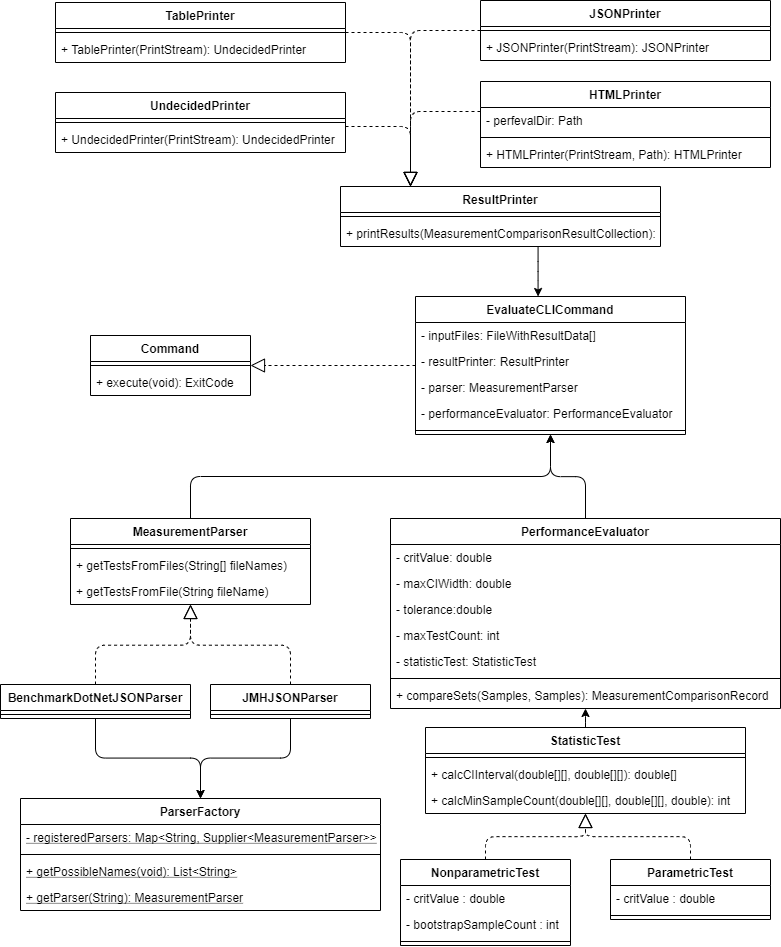
\includegraphics[width=0.92\textwidth]{../img/perfeval_evaluate.png}
    \caption{Objektový návrh části PerfEvalu pro porovnávání výsledků měření}
\end{figure}

\subsection{Inicializace systému PerfEval}

Před použitím systému PerfEval k~vyhodnocování je nutné jej inicializovat.
Účelem inicializace je vytvoření konfiguračního souboru a~databáze pro~ukládání informací o~výsledcích měření.
Tyto soubory jsou potřebné pro fungování systému PerfEval v~rámci vybraného projektu.

Kroky inicializace jsou následující:
\begin{enumerate}
    \item Zjištění zdali adresář podléhá správě verzí systému Git
    \item Vytvoření adresáře .performance
    \item Vytvoření konfiguračního souboru config.ini s výchozími hodnotami
    \item Vytvoření databáze pro ukládání výsledků měření
\end{enumerate}

Při každém spouštění dalšího příkazu systému PerfEval je pak načtena konfigurace z~konfiguračního souboru.
Při vyhodnocování výkonu se načítají výsledky měření společně s~metadaty o~verzi, ke~které se měření vztahuje.
Tato metadata jsou uložena ve~zmíněné databázi.

Pomocí těchto kroků je systém PerfEval inicializován pro~další použití.
Na~následujícím obrázku je vidět objektový návrh části systému PerfEval, která se~stará o~inicializaci systému.
Hlavní třídou je třída \lstinline|InitCommand|, která provádí výše zmíněné kroky inicializace v~rámci metody \lstinline|execute|.
Protože třída inicializace se provádí pomocí příkazu \texttt{init}, tak je třída \lstinline|InitCommand| implementací rozhraní \lstinline|Command|.
Třída \lstinline|PerfEvalConfig| reprezentuje obsah konfiguračního souboru.

\begin{figure}[!ht]
    \centering
    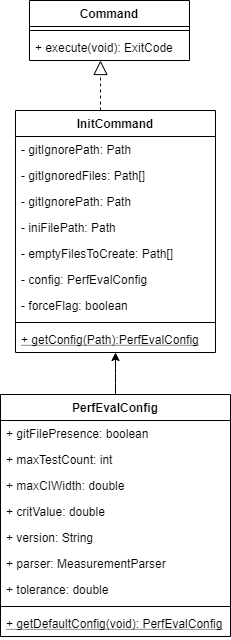
\includegraphics[height=0.5\textheight]{../img/perfeval_init.png}
    \caption{Objektový návrh části PerfEvalu pro inicializaci}
\end{figure}

\subsection{Přidávání nových výsledků testů}

Uživatel musí každý výsledek měření výkonu zaznamenat do~systému PerfEval. Pokud výsledek měření nebude zaznamenán, tak s~ním
PerfEval nebude vůbec pracovat. Přidávat je možné soubory samostatně, nebo z~adresáře. Při~přidávání souborů z~adresáře budou
přidány všechny soubory, a~to i~soubory zanořené ve~vnitřních adresářích zadaného adresáře.

\begin{figure}[!ht]
    \centering
    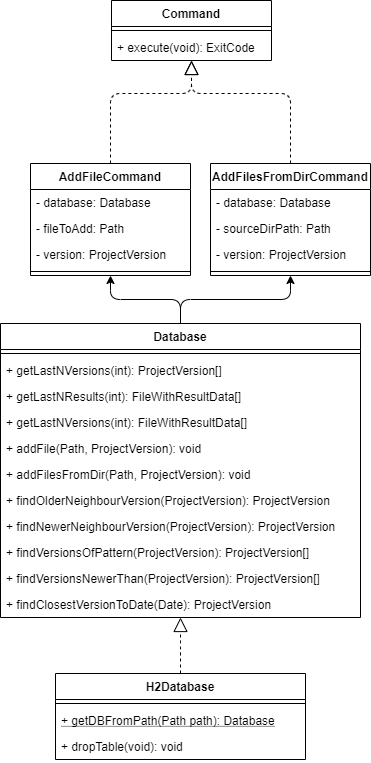
\includegraphics[height=0.5\textheight]{../img/perfeval_h2db.png}
    \caption{Objektový návrh části PerfEvalu pro přidávání výsledků měření}
\end{figure}

Na obrázku je vidět, že za~oběma příkazy pro přidávání výsledků měření stojí jedna implementace rozhraní Database.
Jediná existující implementace tohoto rozhraní využívá technologie H2 databáze. Jedná se o~technologii, která umožňuje
vést si databázi lokálně v~rámci souboru a~pokládat na ní klasické SQL dotazy.

Implementace rozhraní Database pomocí technologie H2 je třída H2Database. V~rámci databáze pro jeden projekt, který
PerfEval spravuje, jsou lokální soubory H2 databáze uloženy v adresáři .performance. Databáze pro správu dat o~výsledcích
měření má jen jednu tabulku. V~této tabulce jsou informace o~cestě k~souboru a~informace o~verzi.

